\chapter{تعریف مساله}

\section{مقدمه}
یکی از نیازمندی‌هایی که در \cite{ETSI-MAN} بیان شده است،
نیاز هر یک از نمونه‌های یک زنجیره‌ی کارکرد سرویس به یک \lr{VNFM}
می‌باشد.
قصد این رساله تعریف مساله‌ای جامع و واقعی است که بتواند این موضوع را نیز در برگیرد
چرا که این نیازمندی برای مراکز داده‌ای بسیار مهم بوده
و در صورت در نظر نگرفتن آن ممکن به کیفیت سرویس آن‌ها لطمه بخورد.
مساله به صورت توامان جایگذاری زنجیره‌ها و \lr{VNFM} برای آن‌ها را مدنظر قرار می‌دهد و
اجازه می‌دهد که سیاست‌های زیر به مساله اعمال شود:

\begin{itemize}
    \item
    برخی از سرورهای فیزیکی ممکن نباید توسط سرورهای فیزیکی مشخصی مدیریت شوند.
    مثلا به علت فاصله زیادی که با یکدیگر دارند یا به علت مسائل امنیتی
    \item
    برخی از کارکردهای مجازی نیاز به سخت‌افزارهای خاصی دارند که ممکن است تنها بتوانند
    بر روی سرورهای فیزیکی مشخصی قرار گیرند.
\end{itemize}

در کنار این سیاست‌ها سعی شده است منابع مدیریتی به صورت کامل مدل‌سازی شوند.
در دنیای امروز برای استفاده از \lr{VNFM}های تجاری نیاز است
که هزینه‌ای پرداخت شود و هر یک از نمونه‌های تهیه شده می‌تواند تعداد مشخصی از کارکردها را مدیریت کند.
در کنار این امر، \lr{VNFM}ها منابع پردازشی مصرف می‌کنند و
نیاز دارند که کارکردهایی که مدیریت می‌کنند در شعاع خاصی از آن‌ها قرار داشته باشند. تمامی این موارد در مساله‌ی طرح شده مدنظر می‌باشند.
این فصل فرمول‌بندی مساله و تنظیمات آن را مرور می‌کنیم و در آخر یک مثال از این مساله را می‌بینیم.
 
\section{مساله}

بیشینه کردن سود حاصل از پذیرفتن تقاضای زنجیره‌ کارکرد سرویس با در نظر گرفتن انتساب هر نمونه کارکرد مجازی شبکه به یک \lr{VNFM}.
همانطور که در مستند \cite{ETSI-MAN} نیز آمده است، نیاز است که هر یک نمونه‌های کارکردهای مجازی شبکه
توسط حداقل یک \lr{VNFM} مدیریت شوند.
در این مساله قصد داریم مساله پذیرش تقاضاهای زنجیره‌های کارکرد سرویس را با نظر گرفتن این نیازمندی در کنار
نیازمندی‌های پردازشی و پهنای‌باند هر یک از تقاضاها حل کنیم.


در ادامه به صورت خلاصه شرایط مساله را بررسی می‌کنیم:

\begin{itemize}
    \item توپولوژی زیرساخت شامل پهنای باند لینک‌ها و ظرفیت \lr{NFVI-PoP}ها\footnote{\lr{NFVI Point of Presence}} موجود است.
    \item \lr{n} تقاضای زنجیره‌ کارکرد سرویس به صورت کامل و از پیش مشخص شده داریم.
    \item هر تقاضا شامل نوع و تعداد نمونه‌های مجازی، پنهای باند لینک‌های مجازی و توپولوژی نمونه‌های مجازی می‌باشد.
    \item \lr{F} نوع کارکرد مجازی شبکه تعریف شده است که هر یک مقدار مشخصی از حافظه و توان پردازشی را مصرف می‌کنند.
    \item تعداد پردازنده‌هایی که به هر نمونه تخصیص می‌یابد با توجه به ترافیک ورودی نمونه مشخص می‌شود. این امر توسط اپراتور در زمان تعریف مساله ورودی صورت می‌گیرد.
    \item نمونه‌ها بین زنجیره‌ها به اشتراک گذاشته نمی‌شوند.
    \item محدودیت ظرفیت لینک‌ها
    \item محدودیت توان پردازش سرورهای فیزیکی با توجه به میزان حافظه و تعداد پردازنده‌ها
    \item برای مدیریت یکدست و آسان‌تر زنجیره‌ها و در عین حال جمع‌آوری راحت‌تر خطاها، برای هر زنجیره یک \lr{VNFM} فیزیکی تخصیص می‌دهیم.
    \item \lr{VNFM}ها می‌توانند بین زنجیره به اشتراک گذاشته شوند.
    \item هر نمونه از \lr{VNFM}ها می‌تواند تعداد مشخصی از نمونه‌های کارکرد مجازی شبکه را سرویس دهد. 
    \item برای ارتباط میان هر نمونه از \lr{VNFM}ها و \lr{VNF}ها پهنای باند مشخصی رزرو می‌گردد.
    \item در صورتی که \lr{NFVI-PoP} بتواند از \lr{VNFM} پشتیبانی نماید می‌توان به هر تعداد که ظرفیت آن اجازه می‌دهد بر روی آن \lr{VNFM} مستقر کرد.
    \item هر نمونه از \lr{VNFM} جهت استفاده نیاز به تهیه جواز\footnote{\lr{license}} دارد.
    \item توپولوژی می‌تواند دارای تعدادی گره‌ی ورودی\footnote{\lr{ingress}} و خروجی\footnote{\lr{egress}} باشد.
    \item هر زنجیره می‌تواند دارای تعدادی نقطه‌ی ورودی و خروجی باشد که می‌بایست بر روی گره‌های ورودی و خروجی نگاشته شوند.
\end{itemize}

اگر جایگذاری \lr{VNFM}ها به صورت غیر برنامه‌ریزی شده صورت بپذیرد
ممکن است به تاخیرهای غیرقابل تحمل منجر شده و به این ترتیب تاثیر منفی بر روی کارآیی سیستم
داشته باشد.

یکی از وظایف \lr{VNFM}ها جمع‌آوری پیام‌های خطا می‌باشد،
برای این امر نیاز است که پهنای باند کوچک اما اختصاصی به \lr{VNFM}ها
تخصیص داده شود بنابراین نمی‌توان جایگذاری آن‌ها را با روش‌های سابق و مانند سایر
کارکردهای مجازی شبکه فرض کرد.

از آنجایی که \lr{VNFM}ها نیاز به مجوز دارند می‌توان با به اشتراک گذاشتن آن‌ها در هزینه‌های سیستم صرفه‌جویی کرد.

در نظرگرفتن \lr{VNFM} همراه با \lr{VNF}ها مساله‌ی جدیدی است.

\section{مدل سیستم}
\subsection{شبکه‌ی زیرساخت}
شبکه‌ی زیرساخت با گراف وزن‌دار
\(G_S^{PN} = (V_S^{PN}, E_S^{PN})\)
نشان داده می‌شود
که در آن
\(V_S^{PN}\)
نشان‌دهنده‌ی مجموعه‌ی گره‌های زیرساخت
و
\(E_S^{PN}\)
نشان‌دهنده‌ی مجموعه‌ی یال‌های شبکه زیرساخت
است.

\begin{itemize}
    \item تمامی گره‌ها مقداری حافظه و تعدادی هسته دارند.
    \item برخی از گره‌ها ممکن است نتوانند توسط گره‌های مشخصی مدیریت شوند.
    \item برخی از گره‌ها ممکن است توانایی پشتیبانی از سرویس‌های مجازی را نداشته باشند.
    \item گره‌های مشخصی در شبکه وجود دارند که می‌توانند در نقش گره‌ی ورودی و خروجی عمل کنند.
    \item یال‌های شبکه همگی دارای ظرفیت مشخصی می‌باشند.
\end{itemize}

\subsection{منابع مدیریتی}
هر یک از
\lr{VNFM}‌ها
نیاز به یک گواهی دارند با مصرف مقدار مشخصی از حافظه و هسته‌های پردازنده
می‌توانند تعداد مشخصی از نمونه‌ها را سرویس دهند.

\subsection{انواع}
هر یک از انواع کارکردهای مجازی شبکه
نیاز به مقدار مشخصی از حافظه و هسته‌های پردازنده دارند
و ممکن است نیازمند مدیریت شدن باشند یا این نیاز را نداشته باشند.
برخی از کارکردها نیاز دارند بر روی نودهای ورودی یا خروجی قرار گیرند.

\subsection{زنجیره‌ها}
زنجیره‌‌ی \(i\)ام با گراف وزن‌دار
\(G^{SFC}_i = (V^{SFC}_{i, F}, E^{SFC}_i)\)
نشان داده می‌شوند
که در آن
\(V^{SFC}_{i, F}\)
نشان‌دهنده‌ی مجموعه‌ی گره‌های زنجیره
و
\(E^{SFC}_{i}\)
یال‌های زنجیره می‌باشد.
تمامی گره‌ها دارای یک نوع مشخص می‌باشند و تمامی یال‌ها ظرفیت مشخصی دارند.

\section{فرمول‌بندی}

هدف اصلی مساله پذیرش بیشترین تعداد تقاضا می‌باشد. در اینجا فرض می‌کنیم پذیرش هر تقاضا سودی منحصر به فرد خواهد داشت.
بنابراین تابع هدف به شکل زیر می‌باشد:

\begin{latin}\begin{align}
    max \sum_{h=1}^{T} c_hx_h - \sum_{w \in V_s^{PN}} licenseFee . \bar{y}_w
\end{align}\end{latin}

\begin{table}[h!]
    \vspace{0.5cm}
    \caption{پارامتر‌های مساله}
    \begin{center}\begin{latin}\begin{tabular}{|c|p{10cm}|}
    \hline
    \(memory(k)\) & required RAM of VNF instance with type \(k\) in GB \\
    \hline
    \(core(k)\) & required CPU cores of VNF instance with type \(k\) \\
    \hline
    \(\hat{memory}\) & required RAM of VNFM in GB \\
    \hline
    \(\hat{core}\) & required CPU cores of VNFM \\
    \hline
    \(capacity\) & maximum number of VNF instances that VNFM can handle \\
    \hline
    \(len(h)\) & number of VNF instances in \(h\)th SFC request \\
    \hline
    \(type(v, k)\) & assuming the value 1 if the VNF instance \(v\) has type \(k\)  \\
    \hline
    \(bandwidth(u, v)\) & required bandwidth in link from VNF instance \(u\) to \(v\) \\
    \hline
    \(\hat{bandwidth}\) & required bandwidth in managmeent link \\
    \hline
    \(radius\) & maximum neighborhood distance for instance management \\
    \hline
    \(licenseFee\) & VNFM license fee that must pay for each VNFM \\
    \hline
    \(vnfSupport(w)\) & assuming the value 1 if the physical server \(w\) can support VNF instances \\
    \hline
    \(isManageable(k)\) & assuming the value 1 if the type \(k\) needs a manager \\
    \hline
    \(notManagableBy(w1, w2)\) & assuming the value 1 if the physical server \(w1\) cannot manage by physical server \(w2\) \\
    \hline
    \end{tabular}\end{latin}\end{center}
\end{table}


\begin{table}[h!]
    \vspace{0.5cm}
    \caption{متغیرهای تصمیم‌گیری مساله (قسمت اول)}
    \begin{center}\begin{latin}\begin{tabular}{|c|p{10cm}|}
    \hline
    \(x_h\) & binary variable assuming the value 1 if the \(h\)th SFC request is accepted; otherwise its value is zero \\
    \hline
    \(y_{wk}\) & the number of VNF instances of type \(k\) that are used in server \(w \in V_s^{PN}\) \\
    \hline
    \(z^k_{vw}\) & binary variable assuming the value 1 if the VNF node \(v \in \cup_{i=1}^{T} V_{i, F}^{SFC}\) is served by the VNF instance of type k in the server \(w \in V_s^{PN}\) \\
    \hline
    \(\bar{y}_w\) & the number of VNFMs (each vnfm has its capacity and license fee) that are used in server \(w \in V_s^{PN} \) \\
    \hline
    \(\bar{z}_{hw}\) & binary variable assuming the value 1 if \(h\)th SFC is assigned to VNFM on server \(w \in V_s^{PN}\) \\
    \hline
    \end{tabular}\end{latin}\end{center}
\end{table}

برای هر نود اندازه‌ی مشخصی از حافظه \lr{RAM}
در نظر گرفته می‌شود که هر نمونه‌ی کارکرد با توجه به نوع آن مقدار مشخصی از این حافظه را مصرف می‌کند.
\lr{VNFM} نیز مقدار مشخصی از حافظه را مصرف می‌کند.

\begin{latin}
    \textit{Node Memory Constraint:}
    \begin{align}
        \sum_{k=1}^F y_{wk} memory(k) + \bar{y_w} \bar{memory} \le N_{ram}^{PN}(w)
        \quad
        \forall w \in V_s^{PN}
    \end{align}
\end{latin}

برای هر نود تعداد مشخصی از هسته‌های پردازنده در نظر گرفته می‌شود که هر نمونه‌ی کارکرد با توجه به نوع آن مقدار مشخصی از این تعداد را مصرف می‌کند.
\lr{VNFM} نیز مقدار مشخصی از تعداد هسته‌های پردازنده را مصرف می‌کند.

\begin{latin}
    \textit{Node CPU Constraint:}
    \begin{align}
        \sum_{k=1}^F y_{wk} core(k) + \bar{y_w} \bar{core} \le N_{core}^{PN}(w)
        \quad
        \forall w \in V_s^{PN}
    \end{align}
\end{latin}

اگر \lr{VNF}, \lr{v}
توسط \lr{VNF instance} نوع \lr{k}
روی سرور \lr{w} سرویس شود می‌بایست
\lr{VNF instance} نوع \lr{k}
روی سرور \lr{w} فعال شود.
توجه شود که
اشتراک گذاری \lr{VNF}ها پشتیبانی نمی‌گردد.

\begin{latin}
    \textit{Service Place Constraint:}
    \begin{align}
        \sum_{v \in \cup_{i=1}^T V_{i, F}^{SFC}} z_{vw}^k \le y_{wk}
        \quad
        \forall w \in V_s^{PN}, \forall k \in [1,\ldots, F]
    \end{align}
\end{latin}

اگر تقاضای \lr{h}ام پذیرفته شده باشد
می‌بایست تمام \lr{VNF node}های آن‌
سرویس شده باشند.
یک \lr{VNF} حداکثر یکبار سرویس داده شود.

\begin{latin}
    \textit{Service Constraint:}
    \begin{align}
        x_h = \sum_{k=1}^{F} \sum_{w \in V_{s}^{PN}} z_{vw}^{k}
        \quad
        \forall v \in V_{h,F}^{SFC}, \forall h \in [1,\ldots, T]
    \end{align}
\end{latin}

اگر تقاضای \lr{h}ام پذیرفته شده باشد
می‌بایست توسط یک \lr{VNFM} سرویس شده باشد.

\begin{latin}
    \textit{Manage Constraint:}
    \begin{align}
        x_h = \sum_{w \in V_{s}^{PN}} \bar{z}_{hw}
        \quad
        \forall h \in [1,\ldots, T]
    \end{align}
\end{latin}

محدودیت ظرفیت سرویس‌دهی \lr{VNFM}
این محدودیت براساس تعداد ماشین‌های مجازی که هر
\lr{VNFM}
سرویس می‌دهد تعیین شده است.
در نظر داشته باشید که ممکن است برخی از انواع
\lr{VNF}‌ها
نیازی به مدیریت شدن نداشته باشند.

\begin{latin}
    \textit{Manage Capacity Constraint \& Manage Place Constraint:}
    \begin{align}
        \sum_{i=1}^{T} \bar{z}_{iw} . (len(i) - \sum_{v \in V_{i, F}^{SFC}} \sum_{k \in [1, \dots, F]} type(v, k) . isManageable(k)) \le capacity . \bar{y}_{w}
        \quad
        \forall w \in V_{s}^{PN}
    \end{align}
\end{latin}

اگر \lr{VNF}، \lr{v} توسط
\lr{instance}
نوع \lr{k} روی سرور \lr{w}
سرویس شود می‌بایست خود از نوع \lr{k} باشد.

\begin{latin}
    \textit{Type Constraint:}
    \begin{align}
        z_{vw}^{k} \le type(v, k)
        \quad
        \forall w \in V_{s}^{PN},
        \forall k \in [1,\ldots, F],
        \forall v \in \cup_{i=1}^T V_{i, F}^{SFC}
    \end{align}
\end{latin}

در صورتی که سرور \lr{w}
توانایی اجرای نمونه‌های \lr{VNF}
را نداشته باشد نباید نمونه‌ای روی آن قرار گیرد.

\begin{latin}
    \textit{VNF support constraint}
    \begin{align}
        \sum_{k \in [1, \dots, F]} y_{wk}  = M . vnfSupport(w)
        \quad
        w \in V_{s}^{PN}
    \end{align}
\end{latin}

برخی از سرورهای نمی‌توانند توسط سرورهای مشخصی مدیریت شوند.
این ویژگی به ادمین شبکه امکان مدیریت بیشتری می‌دهد و او می‌تواند با دست باز تمامی
سیاست‌های مورد نظرش را اعمال نماید.

\begin{latin}
    \textit{Manager to node support constraint}
    \begin{align}
        1 - z_{vw_1}^k + \bar{z}_{hw_2} = 0
        \quad
        & \forall w_1 \in V_s^{PN} \forall w_2 \in V_s^{PN} notManagableBy(w_1, w_2) = 1 \nonumber \\
        & \forall h \in [1,\dots,T],
        \forall v \in V_{h,F}^{SFC},
        \forall k \in [1,\dots,T]
    \end{align}
\end{latin}

\begin{table}[h!]
    \vspace{0.5cm}
    \caption{متغیرهای تصمیم‌گیری مساله (قسمت دوم)}
    \begin{center}\begin{latin}\begin{tabular}{|c|p{10cm}|}
    \hline
    \(\tau^{(u,v)}_{ij}\) & binary variable assuming the value 1 if the virual link \((u,v)\) is routed on the physical network link \((i,j)\) \\
    \hline
    \(\bar{\tau}^{v}_{ij}\) & binary variable assuming the value 1 if the managemnt of VNF node $v$ is routed on the physical network link \((i,j)\) \\
    \hline
    \end{tabular}\end{latin}\end{center}
\end{table}

محدودیت زیر بقای جریان در لینک‌های مورد تقاضای کاربر را تضمین می‌کند.
\begin{latin}
    \textit{Flow Conservation:}
    \begin{align}
        \sum_{(i,j) \in E^{PN}} \tau_{ij}^{(u,v)} - \sum_{(j,i) \in E^{PN}} \tau_{ji}^{(u,v)} = \sum_{k=1}^{F} z_{ui}^{k} - \sum_{k=1}^{F} z_{vi}^{k} \nonumber \\
        \forall i \in V_{S}^{PN}, (u,v) \in E_{h}^{SFC}, h \in [1,\ldots, T]
    \end{align}
\end{latin}

محدودیت زیر بقای جریان در لینک‌های مدیریتی را تضمین می‌کند.
\begin{latin}
    \textit{Management flow Conservation:}
    \begin{align}
        \sum_{(i,j) \in E^{PN}} \bar{\tau}_{ij}^{v} - \sum_{(j,i) \in E^{PN}} \bar{\tau}_{ji}^{v} = \sum_{k=1}^{F} z_{vi}^{k} - \bar{z}_{hi} \nonumber \\
        \forall i \in V_{S}^{PN}, v \in V_{h, F}^{SFC}, h \in [1,\ldots, T]
    \end{align}
\end{latin}

محدودیت ظرفیت لینک‌ها
در نظر داشته باشید که لینک‌های مدیریتی نیز مقدار کمی از پهنای باند را به صورت رزرو شده احتیاج دارند.
\begin{latin}
    \textit{Link Bandwidth Constraint:}
    \begin{align}
        \sum_{v \in \cup_{i=1}^{T} V_{i,F}^{SFC}} \bar{\tau}_{ij}^{v} . \bar{bandwidth} + \sum_{(u,v) \in \cup_{i=1}^{T} E_{i}^{SFC}} \tau_{ij}^{(u,v)} . bandwidth(u,v) \le C_{ij} \nonumber \\
        \forall (i, j) \in E^{PN}
    \end{align}
\end{latin}

شعاع همسایگی تضمین می‌کند که زمان سرویس‌دهی توسط
\lr{VNFM}ها
در یک بازه مشخص (از نظر تعداد گام)
خواهد بود.
\begin{latin}
    \textit{Radius Constraint}
    \begin{align}
        \sum_{(i, j) \in E^{PN}} \bar{\tau}_{ij}^{v} \le radius
        \quad
        \forall v \in \cup_{i=1}^T V_{i, F}^{SFC}
    \end{align}
\end{latin}

\section{مساله‌ی نمونه}

قصد داریم زنجیره‌های زیر شکل \ref{fig.14} را در توپولوژی شکل \ref{fig.15} جایگذاری نماییم.


\begin{figure}[h]
\center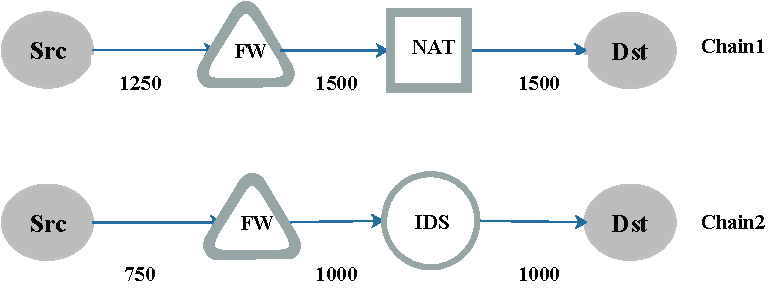
\includegraphics[scale=1]{images/example-chains.pdf}
\caption{زنجیره‌های مساله‌ی نمونه}
\label{fig.14}
\end{figure}


\begin{figure}[h]
\center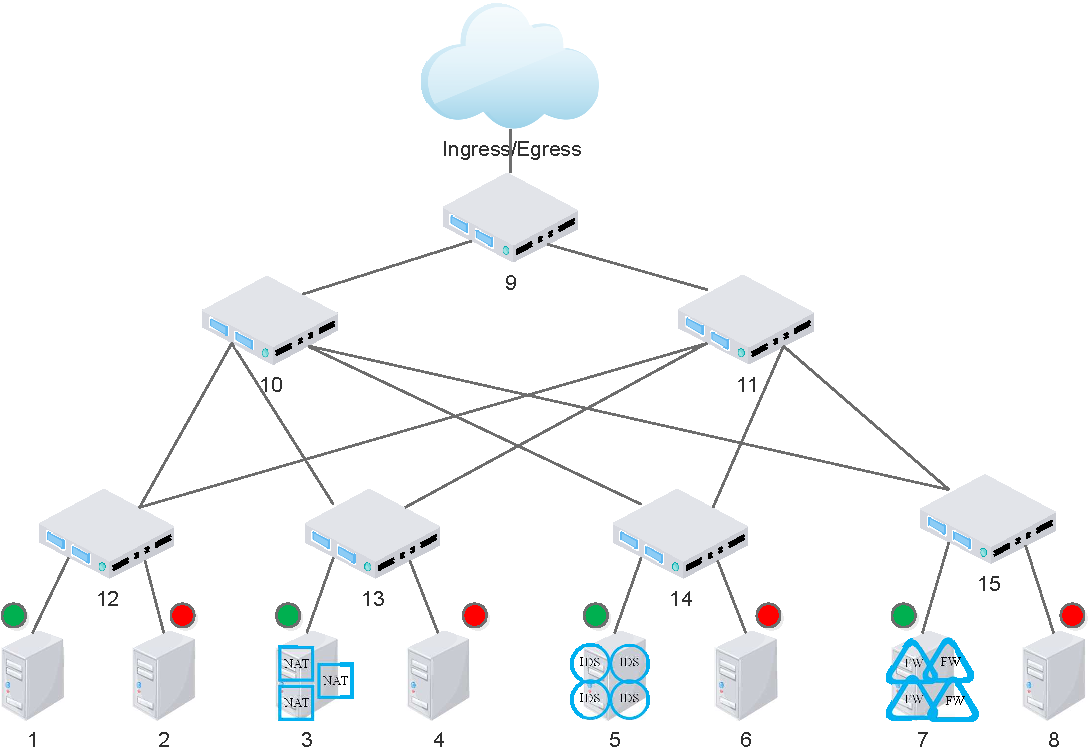
\includegraphics[scale=.75]{images/example-topology.pdf}
\caption{توپولوژی زیرساخت مساله‌ی نمونه}
\label{fig.15}
\end{figure}

نیازمندی‌های نمونه‌ها در شکل \ref{fig.16} آمده است و منابع سرور‌ها نیز در شکل \ref{fig.17} جمع‌آوری شده است.


\begin{figure}[h]
\center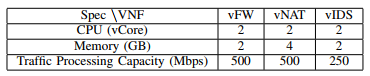
\includegraphics[scale=1]{images/example-types}
\caption{نیازمندی نمونه‌های مساله‌ی نمونه}
\label{fig.16}
\end{figure}

\begin{figure}[h!]
\center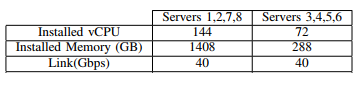
\includegraphics[scale=1]{images/example-spec}
\caption{مشخصات سرورهای زیرساخت مساله‌ی نمونه}
\label{fig.17}
\end{figure}

نمونه‌ها تنها می‌توانند روی سرورهای ۱، ۳، ۵ و ۷ قرار گیرند.
مدیریت سرورهای ۱ و ۳ تنها می‌تواند روی سرورهای ۲ و ۴ انجام شود،
مدیریت سرور ۵ تنها می‌تواند روی سرورهای ۴ و ۶ صورت گیرد
و در نهایت مدیریت سرور ۷ تنها می‌تواند روی سرورهای ۶ و ۸ صورت پذیرد.
هر \lr{VNFM} تنها می‌تواند ۵ نمونه را پشتیبانی کند و
برای این امر نیاز به ۴ گیگابایت حافظه و ۲ هسته‌ی پردازشی دارد.
تمامی لینک‌های فیزیکی ظرفیت ۴۰ گیگابیت بر ثانیه را دارا می‌باشند.

این مثال به صورت کامل بر روی چهارچوب این مساله قابل پیاده‌سازی می‌باشد.

\section{جمع‌بندی}

در این بخش مساله‌ی اصلی بیان شده و شرایط آن شرح داده شد.
فرمول‌بندی مساله در قالب برنامه‌ریزی خطی صحیح مرور شده و در نهایت برای نمایش بهتر مساله یک مثال زده شد.
همانطور که پیشتر همان بیان شده بود مساله قابلیت تنظیم زیادی داشته و این یکی از نوآوری‌های اصلی این رساله می‌باشد.
هدف اصلی مساله نزدیک بودن به واقعیت است و تلاش دارد تمامی سیاست‌های یک مرکز داده‌ای در مساله قابل تنظیم باشند.